\documentclass{beamer}
\usepackage{graphicx}
\title{Team W - Algorithms for Sports Eliminations}
\author{
    Gordon Reid: 1002536R\\
    Ryan Wells: 1002253W\\
    Kristopher Stewart: 1007175S\\
    David Selkirk: 1003646S\\
    James Gallagher: 0800899G\\
    Dr David Manlove: Project Supervisor
}

\date{December 5, 2012}
\begin{document}
\frame{\titlepage}
\frame{\tableofcontents}
\section{Project outline}
\section{Progress so far}
\subsection{Algorithm - Gordon Reid and Ryan Wells}
\subsection{Parser - Kristopher Stewart and James Gallagher}
\subsection{User Interface - David Selkirk}
\frame{
  \frametitle{Project outline}
  \begin{itemize}
  \item<2-> Aim of the project is to implement an algorithm that
  will be able to say that a team X cannot win the Baseball league.
  % Based on schedule of remaining games and current standings.
  \item<3-> Ford-Fulkerson algorithm used.
  % Briefly describe it (?)
  \item<4-> A team X is only eliminated if there is no mathematically possible
  way for X to finish top of the league.
  \item<5-> Builds on na\"{\i}ve calculations made by sports pundits.
  \item<6-> Real world application of Graph Theory.
  \end{itemize}
}
\frame{
  \frametitle{Algorithm}
  \pause
  \begin{center}
  \begin{figure}
  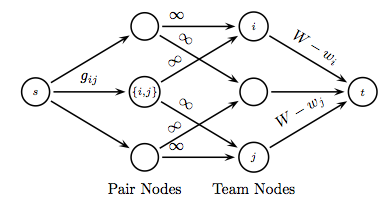
\includegraphics[width=0.4\textwidth]{graph.png}
  \end{figure}
  \tiny{Image courtesy of Kevin D. Wayne, Princeton University}
  \end{center}
  \begin{itemize}
  \item<2-> Revolves around creation of graphs and the flow along them.
  \item<3-> Currently can create all graphs and pushes flow along a particular 
  graph.
  \item<4-> Pushing flow through the graph will allow us to determine if the
  given team X is eliminated from the league.
  \item<5-> A team X can win the league if it is possible for there to be a
  saturating flow. A flow is saturated if the total flow from the source equals
  the total capacity from the source.
  \item<6-> All flow leaving the source has to arrive at the sink.
  \end{itemize}
}
\frame{
  \frametitle{Parser}
  \begin{itemize}
  \item<1-> Currently Parsing a simple .txt file 
  
 \item<2-> Contains all the results from both the National \& American League for the East, Central and West Divisions for 2001 season. 
 \item<3-> Uses basic string comparison to put the relevant team in the correct League and Division. This is Hard coded into the parser. 
 
  \item<4-> Have considered future plans to parse a web page. Be done by looking at the Html of the page, and extracting the relevant data. 
\item<5->Finding the correct page has been proving problematic.
\item<6-> As a team we are unsure if we would like to implement this feature or concentrate our energies on other features.
\item<6->  I.E Making the App web based.    
 
  \end{itemize}
}
\frame{
  \frametitle{User Interface}
  \begin{itemize}
  \item<1-> Shows on slide 1 first
  \item<2-> Shows on slide 2 first
  \end{itemize}
}
\end{document}
